\section{Myo band arm}
%What does the band consist of?
%Electrodes, gyroscope and accelerometer
%Build-in filters and stuff like that?
%Sampling frequency

Myo band arm is a gesture interactive system developed by Thalmic Labs capable of identifying the movement of hands and arms in order to interact and control different electronic devices.

\begin{figure}[H]                    
	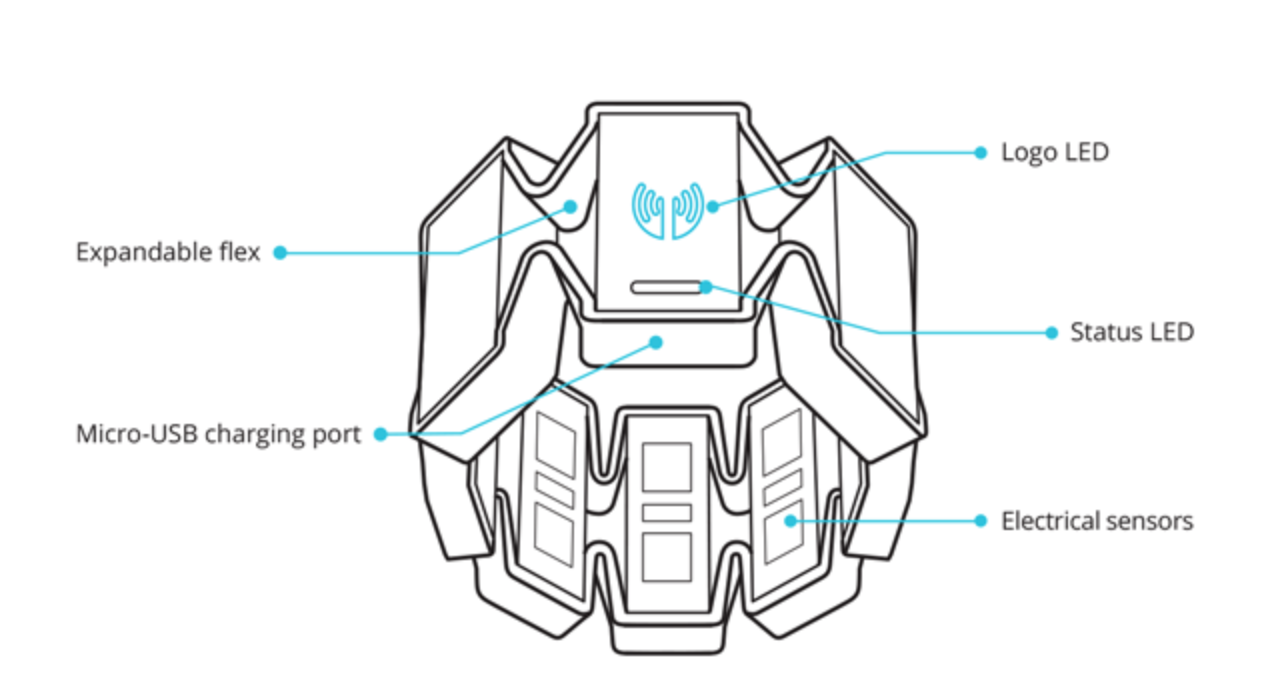
\includegraphics[width=.5\textwidth]{figures/myob/armband}  %<--but is not needed.
	\caption{Main components of the Myo armband. \cite{}}
	\label{fig:armband}  %<--give the figure a label, so you can reference!
\end{figure}


The main components of the Myo armband illustrated in the figure \ref{fig:armband} are:
\begin{itemize}
\item The logo LED gives information about the sync state. The LED is solid when you perform the Sync Gesture successfully and
the Myo armband is synced to your arm. The LED pulses when the armband is not synced.
\item The status LED shows the state of the Myo armband. When it lights up in blue once the Myo armband is connected to a device. 
\item The USB charging port allows to charge the Myo armband battery. 
\end{itemize}
The systems counts with sizing clips, these small pieces give a tighter grip which is more appropriated for smaller arms.

This wearable physical device (arm band positioned in the upper forearm) counts with eight medical grade stainless steel electromyogram (EMG) sensors, responsible of recognizing and performing each gesture. In addition, it has nine axis inertial measurement unit (IMU) which enable the detection of arm movement. IMU includes a three axis gyroscope,  a three axis accelerometer and a three axis magnetometer. It is equipped with an ARM Cortex-M4 microprocessor of low consumption.

\begin{figure}[H]                    
	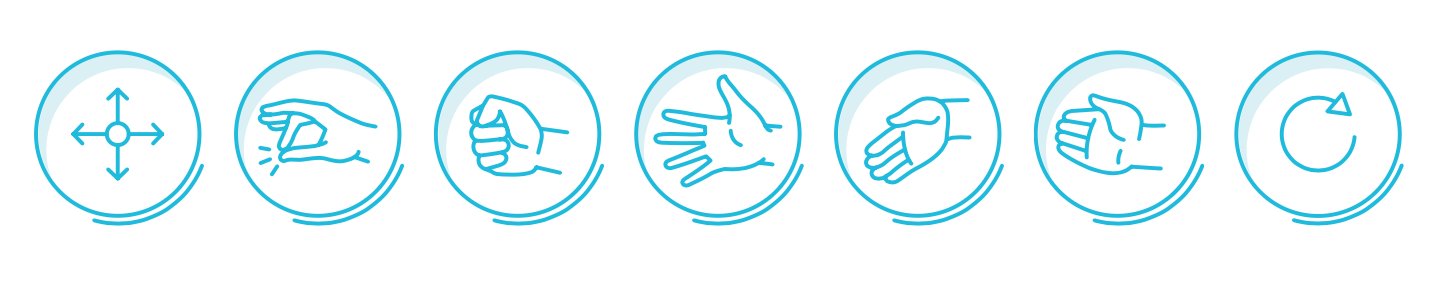
\includegraphics[width=.5\textwidth]{figures/myob/gestures}  %<--but is not needed.
	\caption{Hand gestures detected by proprietary EMG muscle sensors. \cite{}}
	\label{fig:gestures}  %<--give the figure a label, so you can reference!
\end{figure}
It offers five pre-defined gestures as showed in the figure \ref{fig:gestures}, it provides haptic feedback through short, medium or long vibrations to correct moves or activate the system.

The Myo armband is capable of pulling sEMG data at a sample rate of 200Hz while the remaining data (accelerometer, gyroscope and magnetometer) is pulled at a sample rate of  50HZ. The recorded signals can be sent to other devices using Bluetooth 4.0 

Myo band arm supplies two kinds of data:
\begin{itemize}
\item Spatial data, provides information about the orientation and movement of the user's arm. There are two types of spatial data:
\begin{itemize}
\item Orientation
%Orientation
\item Acceleration
\end{itemize}
\item Gestural data which gives information about the user's position of their hands.

\end{itemize}


%/begin{figure}
%poner imagen del los gestos%
%/end{figure}

%How does it communicate with the computer?
%Connection
%Programs that can be used to interface with the arm
%What kind of data will be received from the myo band?


%it connecrs to a PC or tablet via bluetooth Low Energy and allows both raw data streaming and the use of a proprietary library for gesture recognition.The signal processing is performed on the host platform and the used algorithms are not documented (poner de otra manera)


